\chapter{Necesidades y Limitaciones}
En este capítulo, se abordan las necesidades y limitaciones clave que deben considerarse al diseñar y simular un sistema de energía basado en componentes comerciales para globos de gran altitud en ambiente estratosférico. Estas consideraciones son fundamentales para asegurar un funcionamiento óptimo y eficiente del sistema en el desafiante entorno estratosférico. 

\hspace{1.27cm}Comenzaremos explorando las condiciones ambientales específicas a las que se enfrentará el sistema durante su operación en la estratosfera. Estas condiciones incluyen variaciones extremas de temperatura y presiones atmosféricas, entre otros factores, que plantean desafíos significativos en la selección y rendimiento de los componentes utilizados.

\hspace{1.27cm}Además, realizaremos un presupuesto energético del sistema para determinar la cantidad de energía requerida para alimentar el subsistema de telemetría, navegación y carga útil. Este análisis nos permitirá establecer los requisitos de potencia y energía que deben cumplirse, así como identificar oportunidades para optimizar la eficiencia energética y maximizar la autonomía del sistema.

\hspace{1.27cm}Asimismo, examinaremos las limitaciones de masa y volumen a las que el sistema está sujeto. Es esencial diseñar un sistema que cumpla con los requisitos establecidos según el contexto de aplicación, en este caso se evaluarán para la misión StratoBalloon.

\hspace{1.27cm}Adicionalmente, detallaremos de manera concisa las funciones del Sistema de Energía (EPS) y los protocolos de comunicación necesarios para la interconexión con los demás subsistemas de la sonda de HAB. Esto permitirá comprender de forma integral el papel del EPS en el funcionamiento global del sistema.

\hspace{1.27cm}Por último, obtendremos una tabla resumen que recopilará los requerimientos identificados en las secciones anteriores. Esta tabla ofrecerá una visión general y clara de las necesidades y limitaciones del sistema de energía propuesto, así como los mecanismos de verificación.



%REQUERIMIENTOS AMBIENTALES

\section{Condiciones ambientales}

La operación efectiva de un sistema de energía para globos de gran altitud en ambiente estratosférico es fundamental para garantizar el éxito de la misión. Este logro depende en gran medida de la comprensión y abordaje adecuado de las condiciones ambientales a las que estará expuesto.

La utilización de software de predicción de trayectoria es una herramienta esencial en misiones de \emph{High-Altitude Balloons }(HAB), ya que nos permite estimar la zona de aterrizaje, planificar la ruta de vuelo y definir el procedimiento de recuperación. Entre los programas más comúnmente utilizados para esta tarea se encuentran el \emph{Cambridge University Spaceflight} (CUSF) \cite{Cambridge}, \emph{Balloon Trajectory Forecasts} de la universidad de Wyoming \cite{uwyo_balloon_traj} y \emph{Balloon Prediction } \cite{noaa_wvap_sw}. Todos estos simuladores han sido desarrollados basados en el modelo \emph{Global Forecast System} (GFS) de la NOAA \cite{NOAA2023}.

De las alternativas disponibles, hemos decidido utilizar el simulador de la Universidad de Cambridge debido a que nos permite descargar directamente los datos en formato CSV y proporciona información detallada de localización con marcas de tiempo, que será de gran utilidad para nuestro análisis.


\begin{figure}[hbt!]
\centering
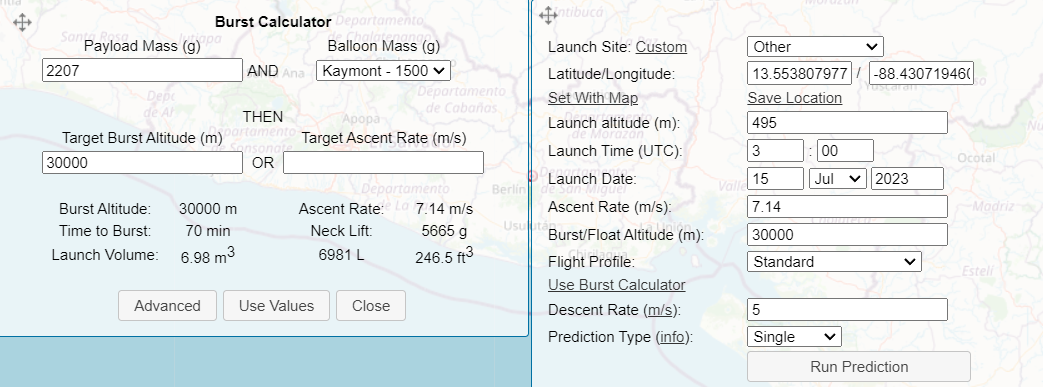
\includegraphics[width=0.75\textwidth]{Pictures/SimulacionParametros.png}
\caption{Valores de entrada para simulador de trayectoria CUSF }\label{fig:SimuladorParametros}
\index{figures}
\end{figure}

\begin{figure}[hbt!]
\centering
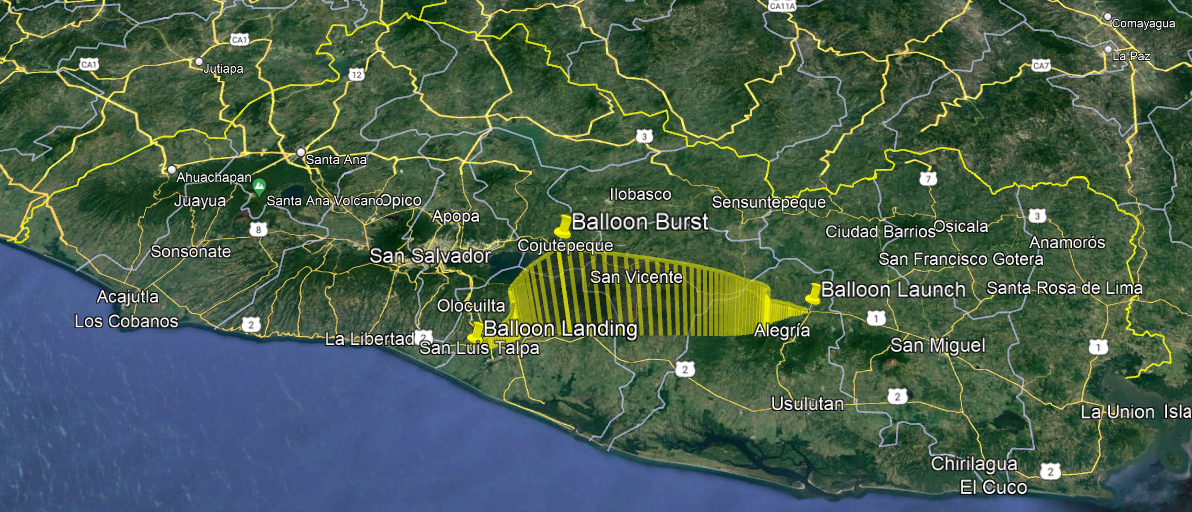
\includegraphics[width=0.75\textwidth]{Pictures/ruta.png}
\caption{Predicción realizada en CUSF visualizada en Google Earth }\label{fig:ruta}
\index{figures}
\end{figure}

Para mejorar nuestra comprensión del comportamiento de variables clave como temperatura y presión durante la misión, es fundamental incorporar el estándar atmosférico ISA en nuestro análisis. El software de CUSF nos ofrece datos de latitud, longitud y altitud, junto con marcas de tiempo con un muestreo cada minuto, lo que facilita la estimación de la duración total de la misión y las razones de cambio en primer y segundo orden para cada variable.

Esta potente combinación nos proporciona una perspectiva más clara y precisa del entorno atmosférico durante todo el vuelo, enriqueciendo significativamente nuestra comprensión de las condiciones ambientales y su evolución en la misión.



\begin{figure}[hbt!]
\centering
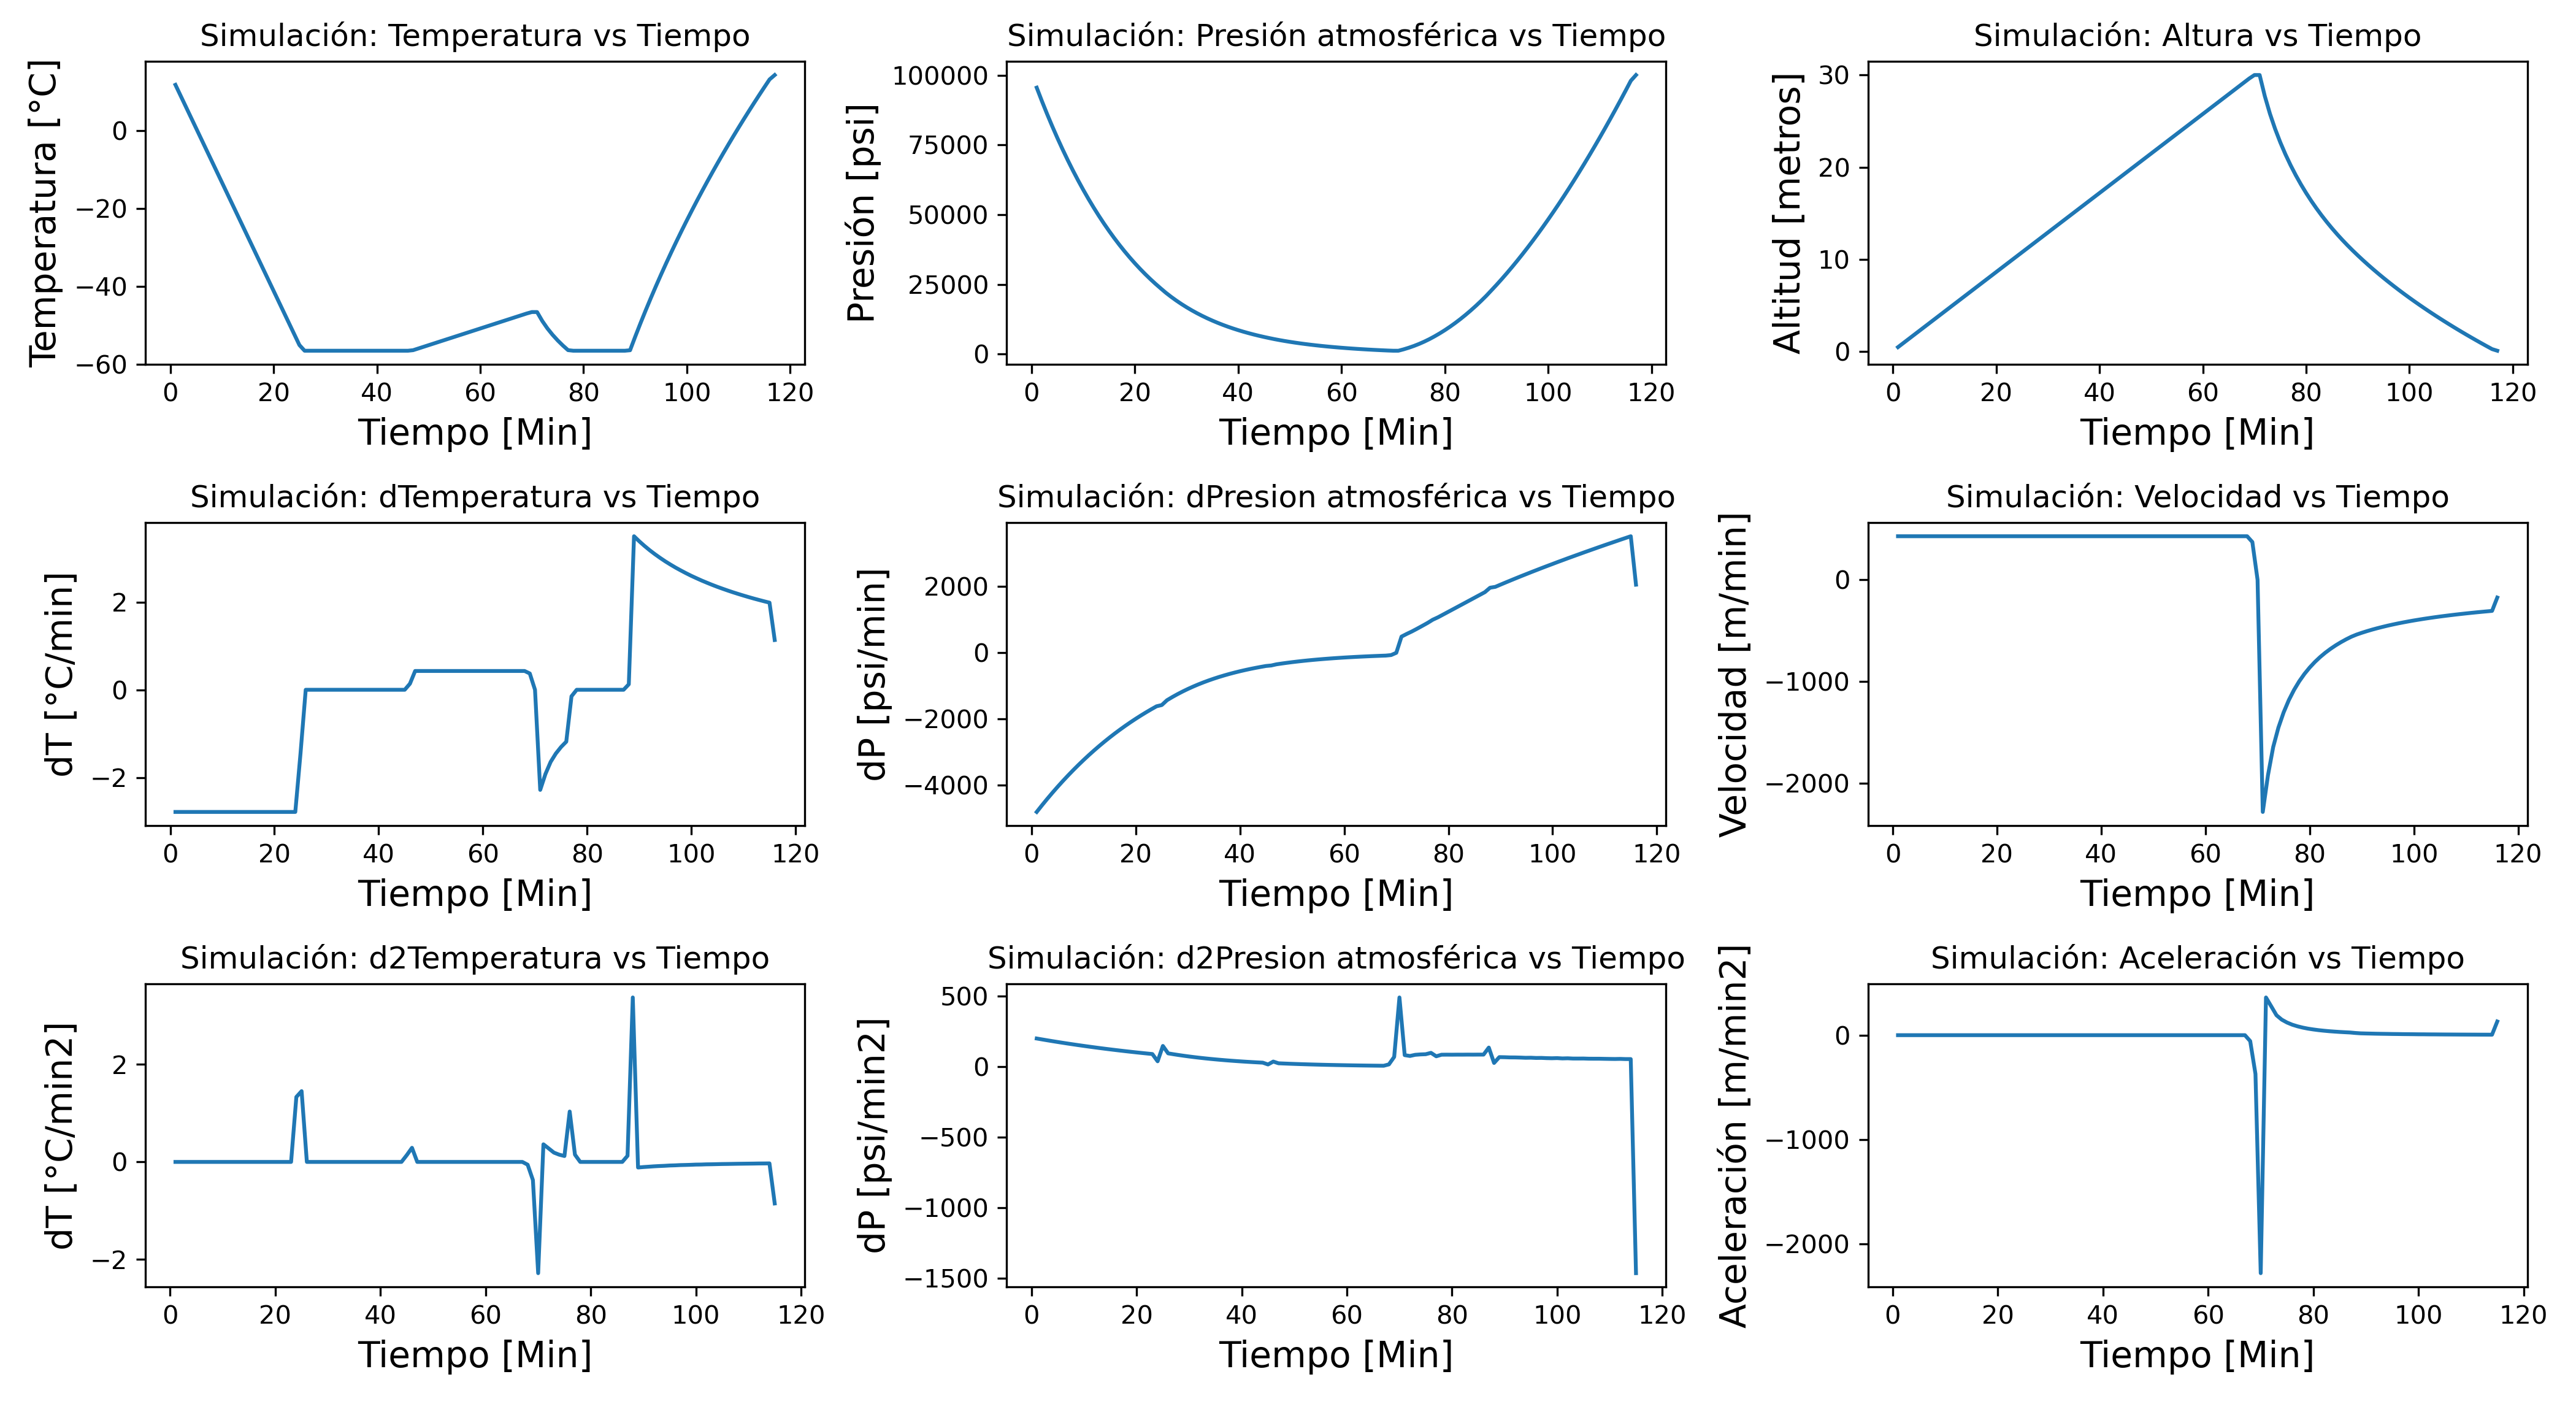
\includegraphics[width=1\textwidth]{Pictures/EnviromentalVariables.png}
\caption{Variables atmosféricas simuladas para una misión de HAB hacia 30 km.}\label{fig:Ambiente}
\index{figures}
\end{figure}

El desarrollo de cálculos en Python desarrollado en trabajos previos  \cite{stratoballoon_eps_batterytest} \cite{osmin-lab} muestra como resultado un comportamiento crítico (ver Fig.\ref{fig:Ambiente}). Las condiciones extremas en la estratósfera pueden alcanzar valores límites de -56.50\degree{}C y 1.20\% de la presión atmosférica estándar. En cuanto a las razones de cambio, se obtuvieron valores máximos de -2.78\degree{}C por minuto y una pérdida de presión atmosférica de 4.74\% por minuto.

Coincidiendo con otros estudios, como el experimento TASEC-Lab \cite{TASEC}, hemos identificado una franja crítica durante el ascenso, alrededor de la tropopausa a 11 km de altitud, con la mayor variación térmica. Este punto es crucial para la selección de componentes y la consideración de sistemas de control térmico.



% Requerimientos Energéticos
\section{Presupuesto energético}

En esta sección, desarrollaremos el presupuesto energético para determinar los requisitos de energía de la misión StratoBallon. La misión se divide en tres subsistemas: telemetría, navegación y carga útil (cámara RGB). Según simulaciones, se estima un tiempo de vuelo promedio de 2 horas para la sonda StratoBalloon. Sin embargo, por seguridad y proceso de recuperación, se añaden 4 horas adicionales, donde solo se requerirá la operación continua de navegación y telemetría.

El presupuesto energético, dividido por bus, se encuentra detallado en las Tablas \ref{tab:cuadro-cargas1} y \ref{tab:cuadro-cargas2}.\\



\begin{table}[!ht]
    \centering
    \renewcommand{\arraystretch}{1.2}
    \caption{Cuadro de cargas para bus 3.3v}
    \label{tab:cuadro-cargas1}
    \begin{tabularx}{1.1\textwidth}{llllllll}
    \hline
    \textbf{Descripción} & \textbf{Cantidad} & \textbf{Susbsistema} & \textbf{I [mA]} & \textbf{P [W]} & \textbf{t [h]} & \textbf{E [Wh]} & \textbf{Q [mAh]} \\
    \hline
    \text{MCU 1} & 1 unidad& Telemetría & 93.00 & 0.31 & 6.00 & 1.84 & 558 \\ 
    \text{LoRa} & 1 unidad & Telemetría & 630.00 & 2.08 & 6.00 & 12.47 & 3780 \\ 
    \text{MCU 2} & 1 unidad & Navegación & 61.00 & 0.20 & 6.00 & 1.21 & 366.00 \\ 
    \text{GNSS} & 1 unidad & Navegación & 100.00 & 0.33 & 6.00 & 1.98 & 600.00 \\ 
    \text{RTD} & 1 unidad & Navegación & 3.50 & 0.01 & 6.00 & 0.07 & 21.00 \\ 
    \text{IMU} & 1 unidad & Navegación & 0.60 & 0.00 & 6.00 & 0.01 & 3.60 \\ 
    \text{MCU 3} & 1 unidad & Carga útil & 70.00 & 0.23 & 2.00 & 0.46 & 140.00 \\ 
    \text{Cámara IR} & 1 unidad & Carga útil & 25.00 & 0.08 & 2.00 & 0.17 & 50.00 \\\hline 
    & & \textbf{I Máx.} & \text{983.10} & & & & \textbf{5518.6} \\ \hline
    \end{tabularx}
\end{table}

\begin{table}[!ht]
    \centering
    \renewcommand{\arraystretch}{1.2}
    \caption{Cuadro de cargas para bus 5.0v}
    \label{tab:cuadro-cargas2}
    \begin{tabularx}{1.1\textwidth}{llllllll}
        \hline
        \textbf{Descripción} & \textbf{Cantidad} & \textbf{Subsistema} & \textbf{I [mA]} & \textbf{P [W]} & \textbf{t [h]} & \textbf{E [Wh]} & \textbf{Q [mAh]} \\
        \hline
        RTC & 1 unidad & Navegación & 0.30 & 0.00 & 6.00 & 0.01 & 1.80 \\
        Buzzer & 1 unidad & Navegación & 24.00 & 0.12 & 6.00 & 0.72 & 144 \\
        Barómetro & 1 unidad & Navegación & 0.00 & 0.00 & 6.00 & 0.00 & 0.00 \\
        MUX & 1 unidad & Navegación & 100.00 & 0.50 & 6.00 & 3.00 & 600 \\
        Datalogger 1 & 1 unidad & Navegación& 6.00 & 0.03 & 6.00 & 0.18 & 36 \\
        Cámara & 1 unidad & Carga útil & 260.00 & 1.30 & 2.00 & 2.60 & 520 \\
        Datalogger 2 & 1 unidad & Carga útil & 12.00 & 0.06 & 2.00 & 0.12 & 24\\\hline
        ~ & ~ & \textbf{I Máx.} & \text{402.30} & ~ & ~ & ~ & \textbf{1325.8} \\
        \hline
    \end{tabularx}
\end{table}



% REQUERIMIENTOS DE MASA Y VOLUMEN

\section{Limitaciones de Masa y Volumen}

El diseño del EPS para la misión StratoBalloon se ve restringido por el contexto de la tesis y la fase avanzada de la misión. Las dimensiones y materiales de la estructura impresa ya han sido definidos \cite{barahona2022diseno}. Los componentes electrónicos de los otros subsistemas también han sido seleccionados, determinando el espacio disponible.

El módulo central (Fig. \ref{fig:imagen1}) reserva dos niveles inferiores estratégicamente ubicados para el EPS, separados por una distancia uniforme de 2.54 cm (Fig. \ref{fig:imagen2}), basada en las medidas detalladas en la Fig. \ref{fig:PlanoPCB}.

Es importante destacar que el peso máximo asignado al EPS en esta misión es de 600 gramos.



\begin{figure}[b]
  \centering
  \begin{subfigure}[b]{0.35\textwidth}
    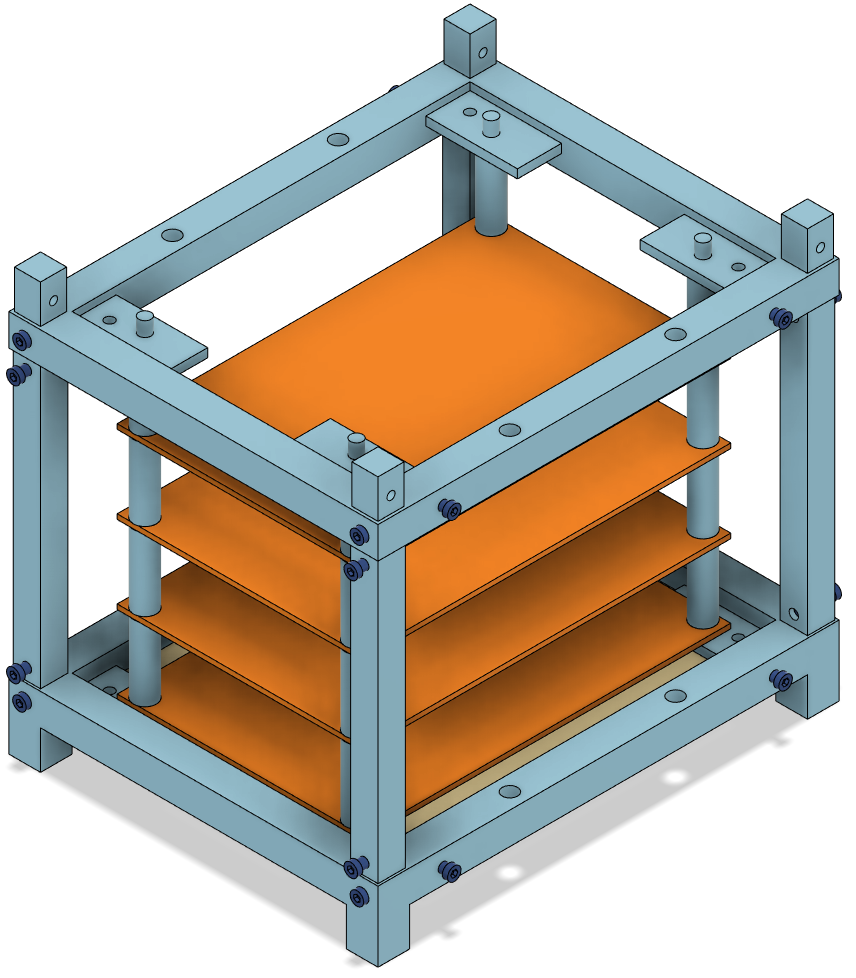
\includegraphics[width=\textwidth]{Pictures/3DPrinting.png}
    \caption{Vista 1}
    \label{fig:imagen1}
  \end{subfigure}
  \hfill
  \begin{subfigure}[b]{0.40\textwidth}
    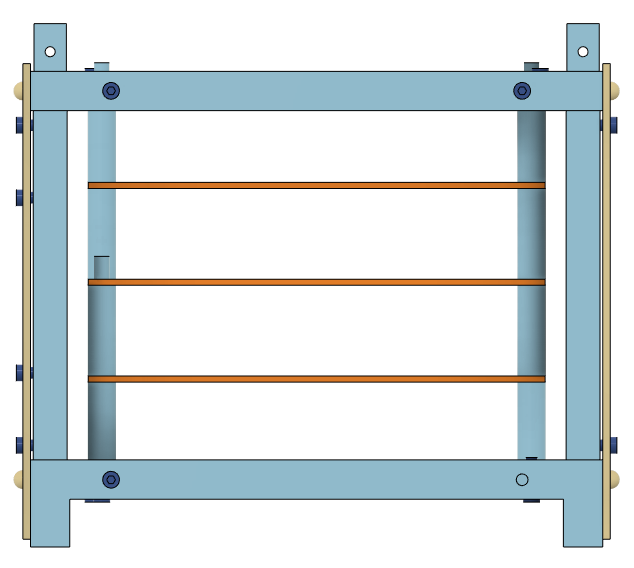
\includegraphics[width=\textwidth]{Pictures/Lateral3DPrinting.png}
    \caption{Vista 2}
    \label{fig:imagen2}
  \end{subfigure}

  \caption{Estructura de impresión 3D}
  \label{fig:dos_imagenes}
\end{figure}
\begin{figure}[hbt!]
\centering
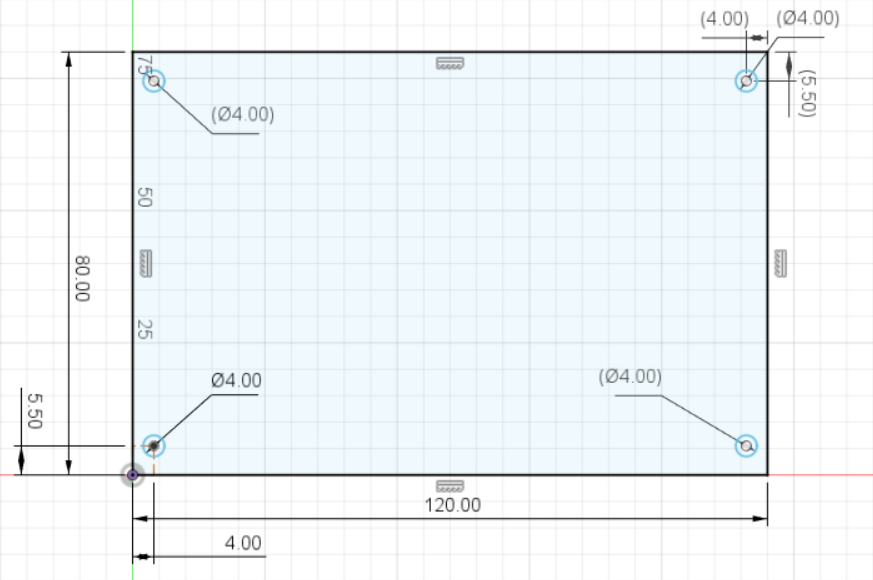
\includegraphics[width=0.75\textwidth]{Pictures/PlanoC.png}
\caption{Dimensiones de PCB en [mm]}\label{fig:PlanoPCB}
\index{figures}
\end{figure}

% RESUMEN DE REQUERIMIENTOS
\section{Resumen de requerimientos}
\vspace{0.5 cm}

El EPS cumple sus funciones principales durante la misión y permite la adquisición de datos para análisis posteriores. A continuación, se detallan los requerimientos del EPS en la Tabla \ref{tab:requerimientos-eps}.

\begin{table}[!ht]
    \centering
    \renewcommand{\arraystretch}{1.2}
    \caption{Requerimientos del EPS}
    \label{tab:requerimientos-eps}
    \begin{tabular}{l|p{4.8cm}|p{4.8cm}|p{4.8cm}}
    \hline
    \textbf{ID} & \textbf{Descripción} & \textbf{Justificación} & \textbf{Mecanismo de verificación} \\
    \hline
    R1 & Resistencia al vacío térmico, temperatura mínima de hasta -56.50°C y 1.20\% de presión atmosférica.& Resultados en simulaciones. & Ensayos en cámara de vacío térmico (Ver a detalle en Anexo \ref{ap:vaciotermico})
 \\
    \hline
    R2 & El EPS debe proveer una línea de alimentación de 3.3 V $\pm$ 1\% con una corriente mínima de 983.1 mA $\pm$ 1\%. & Bus de alimentación. & Medición de V y I.\\
    \hline
    R3 & El EPS debe proveer una línea de alimentación de 5.0 V $\pm$ 1\% con una corriente mínima de 402.30 mA $\pm$ 1\% & Bus de alimentación. & Medición de V y I. \\
    \hline
    R4 & No debe exceder una masa de 600 g. & Limitación de masa. & Medición de masa. \\
    \hline
    R5 & 2 PCB de 12x8 cm con 2.5 cm de altura.  & Limitación de espacio. & Medición de longitud.\\
    \hline
    R6 & Registro de V \text{[v]} y I \text{[mA]}. & Función deseable. & Ensayo de registro de datos. \\
    \hline
    R7 & Registro de T [\text{\textdegree{}C}] y P\text{ [atm]}.  & Función deseable. & Ensayo de registro de datos. \\
    \hline
    R8 & Comunicación I2C. Recepción desde Navegación de la señal de control ON/OFF de carga útil. Transmisión de SoC a telemetría.& Integración de subsistemas. & Ensayo de comunicación. \\
    \hline
    R9 & Control ON-OFF: carga útil.& Ahorro de energía. & Ensayo de control ON-OFF. \\
    \hline
    R10 & Interruptor RBF (Remove before flight, retirar antes del vuelo) para encendido y apagado del EPS.& Seguridad de la Misión, útil para prevenir accidentes. & Medición de continuidad. \\\hline
    R11 & Cargador de baterías con fuente de alimentación VDC externa & Carga del banco de baterías & Medición de voltaje. \\
    \hline
    \end{tabular}
\end{table}





